
\section{Rappel sur la géodynamique de l'atmosphère terrestre}%
\label{sec:structure_atmosphere}

\subsection{Composition chimique de l'atmosphère}%
\label{ssub:composition_chimique_de_latmosphere}

L'atmosphère de la terre est composée principalement de gas. Sa composition sèche est
faite d'diazote \ce{N2} à \SI{78.087}{\percent}, de dioxygène \ce{O2} à
\SI{20.95}{\percent}, argon \ce{Ar} à \SI{0.93}{\percent}. Parmis les pourcentages restant
se trouvent le dioxide de carbone \ce{CO2} (\SI{0.041}{\percent}) et le methane \ce{CH4},
en augmentation depuis le début de l'activité industrielle, ainsi que d'autres gas à
l'état de trace (néon \ce{Ne}, hélium \ce{He} et krypton \ce{Kr}).  Cette composition est
dite ''sèche'' car ne prend pas en compte la vapeur d'eau, représenant en moyenne 
\SI{0.25}{\percent} de la masse total de l'atmosphère, mais en quantité extrèmement
variable selon la localité géograhique ou temporelle.

De plus, sous l'effet des radiations solaire et notamment les longeurs d'ondes
ultra-violettes (UV), de nombreux radicaux hydroxyle \ce{HO^.} sont formés et réagissent
rapidement avec les autres composants de l'atmosphère.  La quantité de dioxygène et la
présence de radicaux hydroxyle, entre autre, font de l'atmosphère un milieu a grande
capacité oxydante ayant un impact directe sur les différentes réactions pouvant avoir lieu,
aussi bien avec les gas à effet de serre que pour les polluants organiques présent dans
les basses couches de l'atmosphère.

Enfin, il est à noté que l'atmosphère n'est pas composé que de gas mais également de
particule solide ou liquide en suspension, que ce soit des critaux de glace ou d'eau
liquide sous forme de nuage, mais également de ''poussières'', dont il sera question dans
cette thèse, et qui seront plus explicitement détaillé
ci-après~\ref{sec:les_aerosols_atmosphereiques}.

\subsection{Structuration de l'atmosphère}%
\label{sub:structuration_de_l_atmosphere}

\subsubsection{Une organisation stratifiée}%
\label{ssub:une_organisation_stratifiée}

À première vue l'atmosphère terrestre peut sembler homogène depuis le sol jusqu'à
l'espace. En réalité, de grande hétérogénéitées sont observées à certaines altitudes,
formant des couches concentriques aux propriétés physico-chimique très différentes, ne se
mélangeant que peu, limitant ainsi les échanges entre elles (voir
Figure~\ref{fig:chapter01/Comparison_US_standard_atmosphere_1962}).

Notamment, c'est dans la première strate atmosphérique, de \SI{0}{km} à \SI{13}{km} en
moyenne, la troposphère, que se déroule les phénomènes météorologiques
"directement sensible" au quotidien
(convection, formation de nuages, transport longue distance de poussières…).
C'est également la troposhère qui totalise près de \SI{75}{\percent} de la masse totale
de l'atmosphère, mais surtout en ce qui nous intéresse dans cette thèse, qui contient la
quasi totalité de l'eau et des aérosols.

La tropopause marque la séparation entre la troposhère et la stratosphère. Elle est
notable par son changement brutale de gradient thermique (\SI{-6}{\degreeCelsius\per\km}
dans la troposhère, à \SI{0}{\degreeCelsius\per\km} dans la bas de la stratosphère).
Ceci conduit à une inversion thermique très forte, faisant de la tropopause une véritable
barrière physique. La présence de la couche d'ozone (\ce{O3}) dans la stratosphère
protège la surface de la Terre d'une partie des UV provenant du soleil, en absorbant ces
radiations. Du fait de cette absorption par l'ozone, la stratosphère se réchauffe
progressivement avec l'altitude, jusqu'à arriver à une nouvelle frontière : la
stratopause, marquée par un gradient proche de 0.

Vient ensuite la mésosphère, dénuée d'ozone et présentant donc un refroidissement car au
contact du froid de l'espace. Puis la thermosphère, qui sous l'effet des radiations
solaires, formé des ions par photodissociation, réchauffe cette zone de l'atmosphère.
C'est également à cette altitude que se produissent les aurores-boréales, lorsque les
particules du vent solaire se heurtent au champs électromagnétique terrestre à environ
\SI{100}{km} d'altitude. Puis vient l'espace extra-terrestre après \SI{600}{km}
d'altitude.

\begin{figure}[ht]
    \centering
    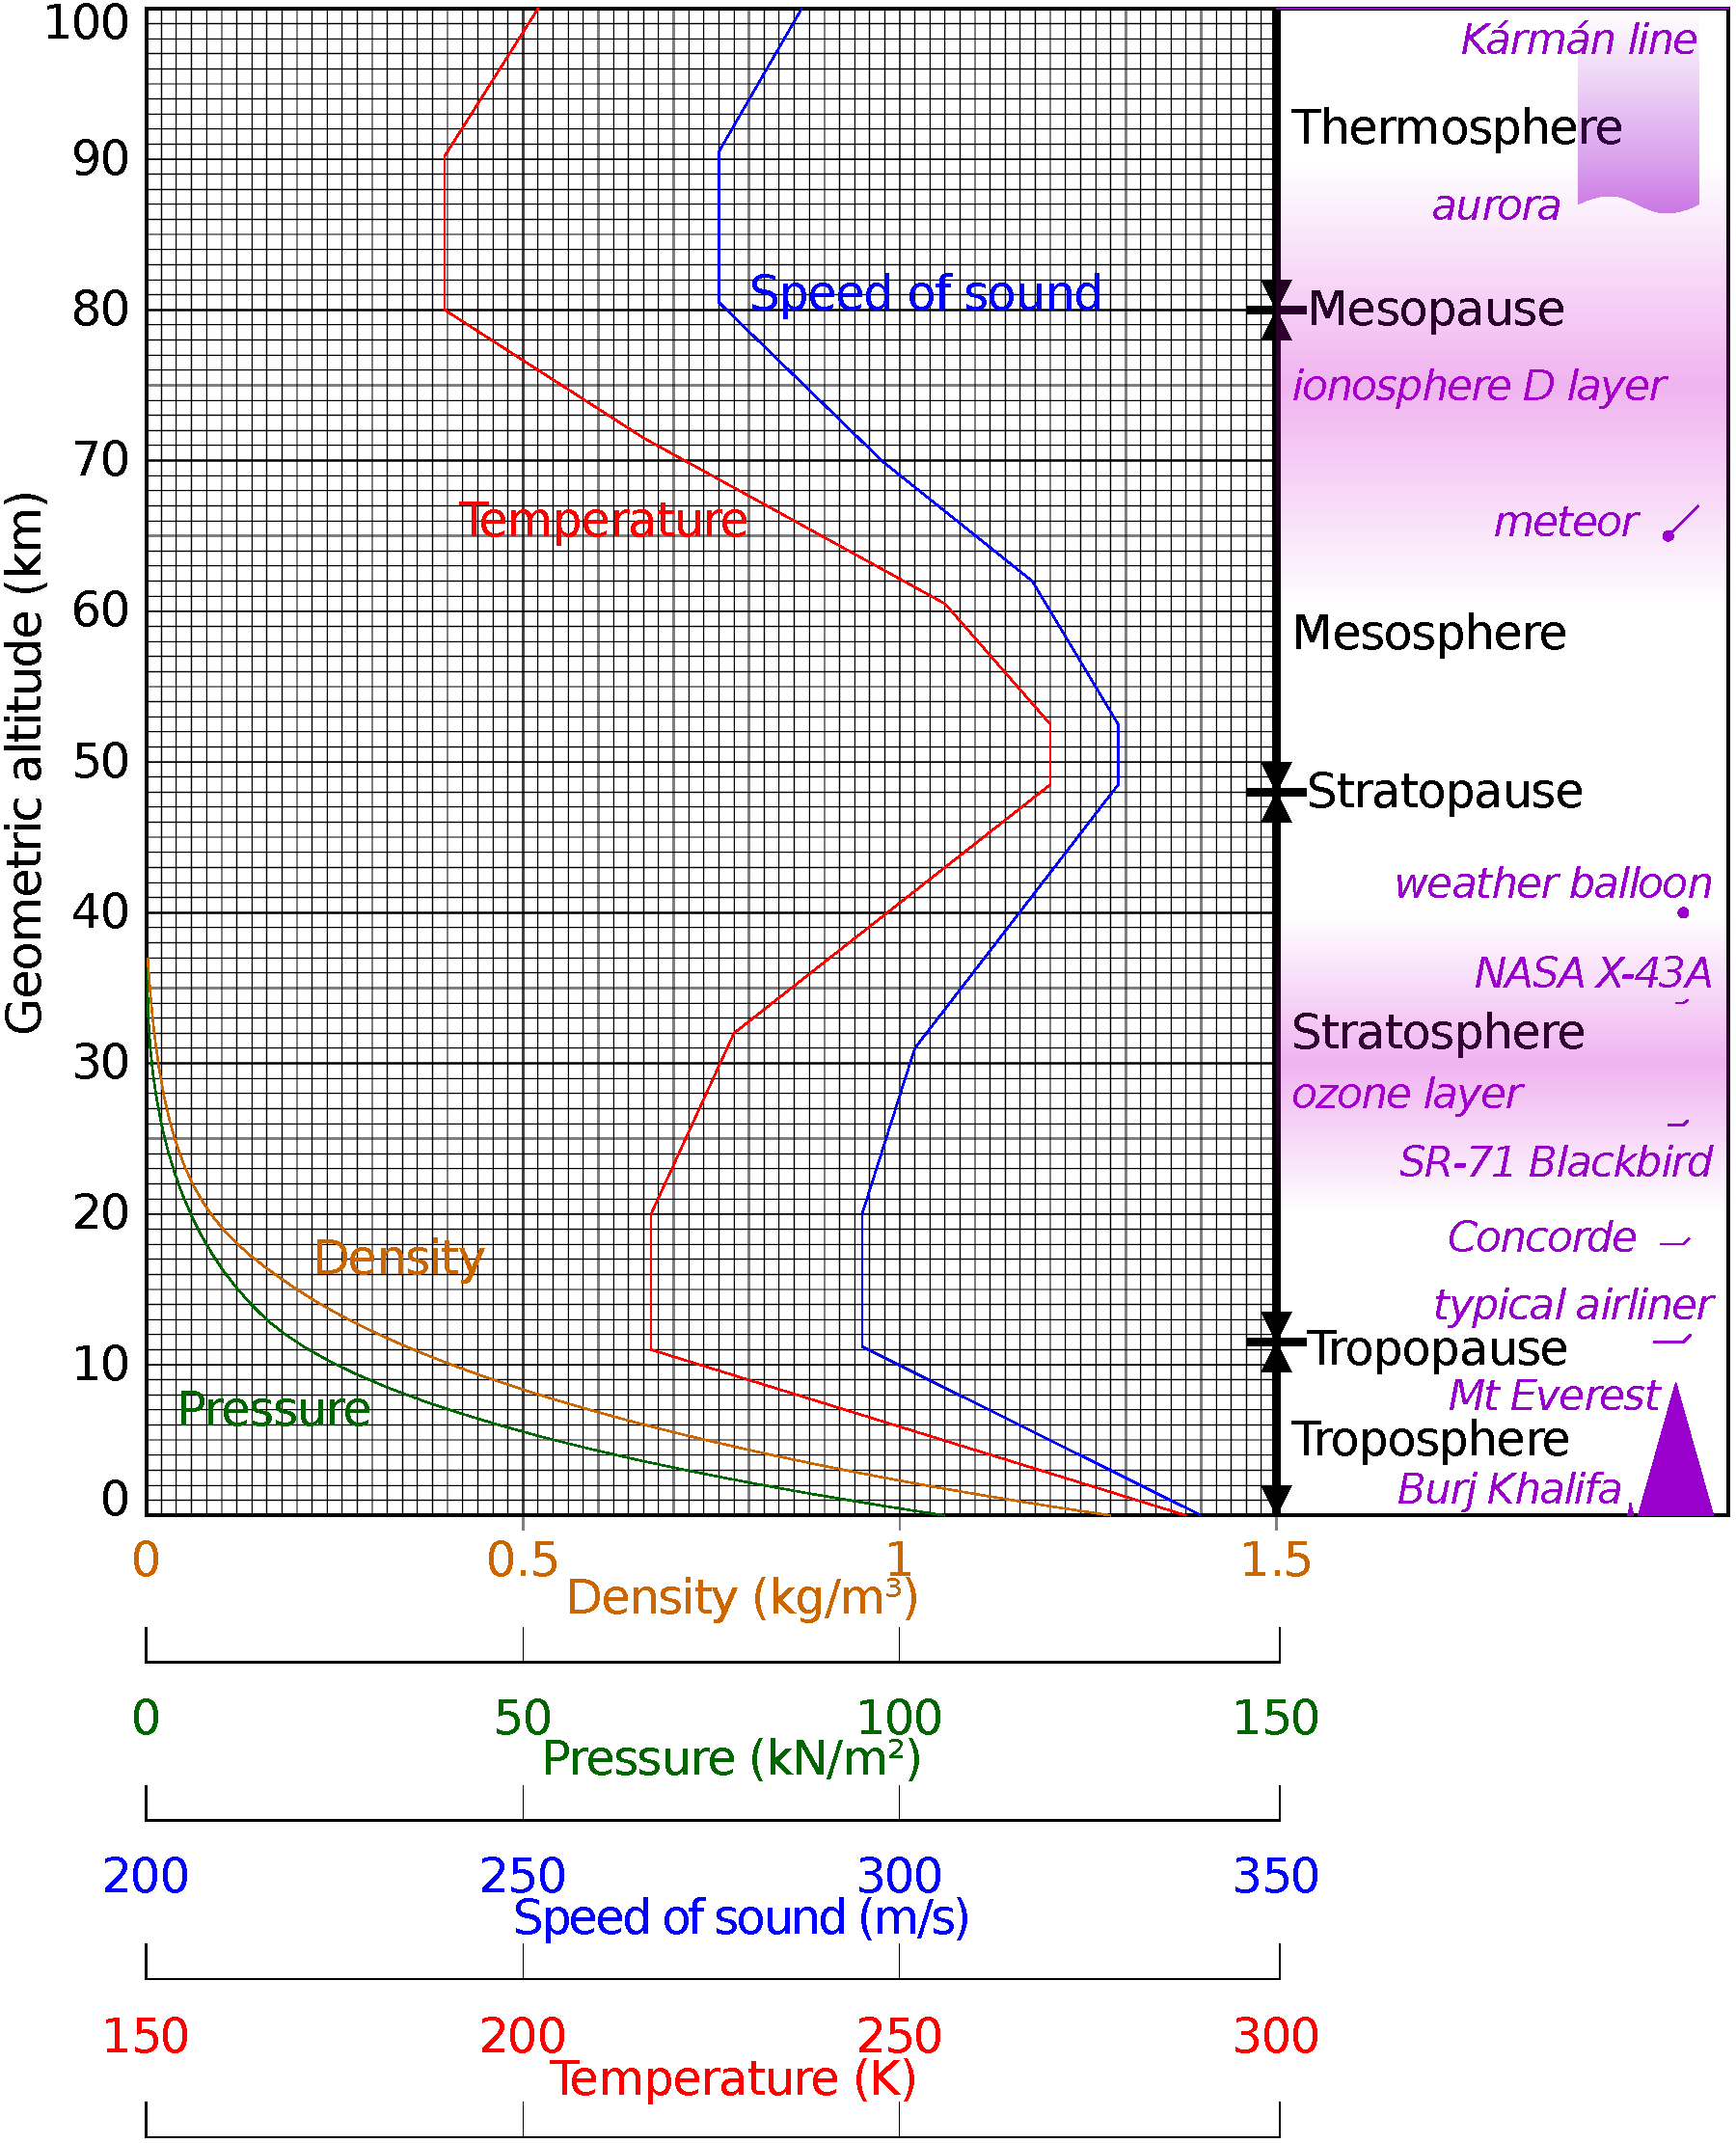
\includegraphics[width=0.6\linewidth]{chapter01/Comparison_US_standard_atmosphere_1962.pdf}
    \caption{%
        Comparaison des variables atmosphèriques selon l'atmosphère standard défini par
        l'\textit{US standard atmosphere} de 1962.
        Source:
        \href{https://commons.wikimedia.org/wiki/File:Comparison_US_standard_atmosphere_1962.svg}{wikicommons},
        par \href{https://commons.wikimedia.org/wiki/User:Cmglee}{Cmglee}, CC-BY-SA.
    }%
    \label{fig:chapter01/Comparison_US_standard_atmosphere_1962}
\end{figure}

\subsubsection{La couche limite atmosphérique}%
\label{sub:la_couche_limite_atmospherique}

À l'interrieur de cette fine couche d'environ \SI{600}{km}, seule la troposhère,
c'est-à-dire les 13 premiers kilomètres, nous est directement familière. C'est en effet
dans la troposhère que les phénomènes météorologiques auquels nous sommes habitués s'y
déroulent : nuage, vent, pluie, etc. Alors que l'atmosphère parait immense, il est
important de noter la faible hauteur de cette couche.

La partie de la troposphère directement impactée par les effets de la surface terrestre
(friction, réchauffement, turbulence) est la couche limite atmosphèrique (CLA, ou
\textit{atmospheric boundary layer (ABL))}. Cette couche de quelques dizaines à centaines
de mètres, selons les lieux et période de la journée, a une dynamique rapide et
convective. En ce qui nous intéresse dans cette thèse, cela a pour conséquences que les
émissions de surface anthropiques ou naturelles, et notamment les polluants, seront
redistribués sur l'intégralité de cette hauteur.

Notamment, durant la nuit, la hauteur de la CLA est faible du fait de l'affaiblissement du
gradient thermique vertical lié à l'absence de réchauffement radiatif du sol (voir
Figure~\ref{fig:chapter01/Atmospheric_boundary_layer} et la mise en place de la couche de
surface après le couché du soleil). Après le levé du soleil, la surface se réchauffe et la
convection se met en place, rendant la CLA beaucoup plus homogène et diluant gaz et
particules dans un plus gros volume d'air. Les composés ne traverse cependant que
rarrement la couche d'inversion thermique, limite entre la CLA et la troposphère libre.
Ainsi, après le couché du soleil, on observe fréquement une couche résiduelle au milieu de
la CLA qui "capture" les composés d'une journée à une autre.

Il est à noter que des couches d'inversions thermiques à plus basse altitude peuvent se
mettre en place, notamment dans les vallées alpines. Pour un flux d'émission
constant, cela entrainne donc une accumulation forte des composés chimiques dans un volume
très restreint, augmentant mécaniquement les concentrations.
\textcite{allardQualite2018} a ainsi pu montrer que le gradient thermique est l'un facteur
explicatif les plus importants pour la compréhension de la compréhension des
concentrations en vallées alpines.
%Notamment, certains jours à Passy, France, un facteur de concentration de 700 était présent entre 

\begin{figure}[h]
    \centering
    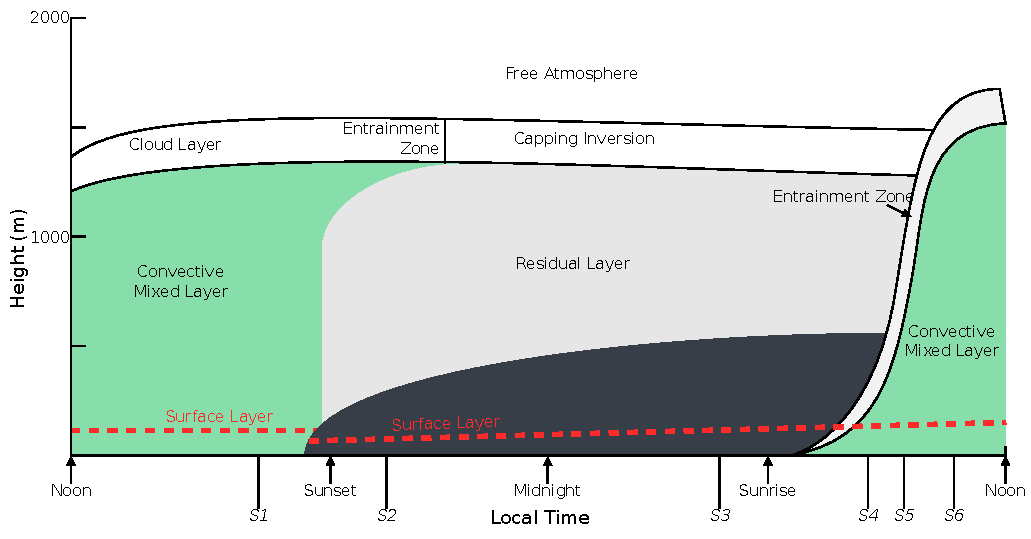
\includegraphics[width=0.8\linewidth]{chapter01/Atmospheric_boundary_layer.pdf}
    \caption{Évolution journalière schématique de la couche limite atmopshèrique.
        Credit: By
        \href{https://commons.wikimedia.org/w/index.php?curid=18862904}{NikNaks} - Own
        work based on:
        \url{http://ars.sciencedirect.com/content/image/1-s2.0-S0360128504000371-gr4.jpg}.
        See also: \url{http://www.archaeocosmology.org/eng/tropospherelayers.htm}., CC
        BY-SA 3.0
    }%
    \label{fig:chapter01/Atmospheric_boundary_layer}
\end{figure}


\section{Les aérosols atmospheriques}%
\label{sec:les_aerosols_atmospheriques}

\subsection{Qu'est-ce qu'un aérosol?}%
\label{sub:quest-ce-quun-aerosol}

L'air que nous respirons est constitué majoritairement de gas (\ce{N2}, \ce{O2}…) mais
également de particule solide ou liquide en suspension dans l'air. Ces particules, très
légères et de taille micrométriques ou moins, constituent une famille de composé appellé
communément particule fine, \textit{particulate matter} (PM) ou improprement particule
diesel dans le grand public.

Leur taille varient de quelques nanometres à plusieurs dizaines de micromètres.
À titre de comparaison, cela reviendrait à mettre dans la même catégorie une marche de
\SI{100}{m} pour aller chercher son pain à un voyage de \SI{10000}{km}.
Ainsi, cette nomenclature ''PM'' regroupe nécessairement des objets aux caractéristiques
très diverses. En effet, comme le montre la Figure~\ref{fig:aerosolDistribution}, selon
que l'on observe les PM en s'intéressant à leur nombre, surface ou volume, l'importance
relative des classes de tailles change complètement.
\begin{figure}[ht]
    \centering
    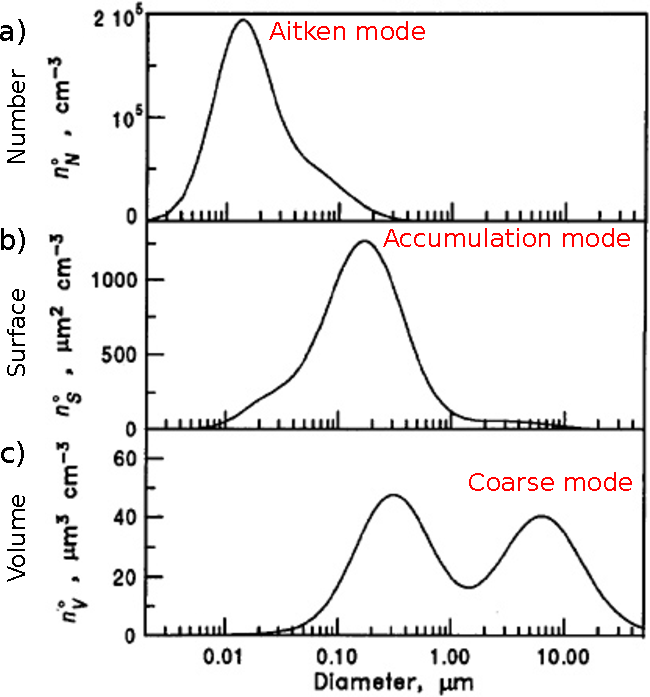
\includegraphics[width=0.5\textwidth]{aerosolDistribution.pdf}
    \caption{Distribution \textbf{(a)} en nombre, \textbf{(b)} surface, et
        \textbf{(c)} volume, pour un ensemble typique de distribution trimodale
        d'aérosols. Figure adaptée du livre de~\textcite{seinfieldAtmospheric1998}.}
    \label{fig:aerosolDistribution}
\end{figure}

La nomenclature des aérosols est ainsi historiquement fondé sur leur taille:
\begin{itemize}
    \item \PMdix, dont le diamètre aérodynamique inférieur ou égal à \SI{10}{\um}
    \item \PMdc, dont le diamètre aérodynamique inférieur ou égal à \SI{2.5}{\um}
    \item \PMun, dont le diamètre aérodynamique inférieur ou égal à \SI{1}{\um}
\end{itemize}

Ces différents modes reflètes différents procédés conduisant à leur présence dans l'air,
allant de la nucléation à partir de composé gaseux ou de source de combustion pour le mode
dit d'Aikten, le plus fins (prépondérant en nombre), permettant par coagulation
d'atteindre des particules plus grosses (mode d'accumulation) allant jusqu'au \PMdc, pour
enfin, lorsque la vitesse de coagulation est suffisante, atteindre le mode grossier
\PMdix, pouvant également être allimenté par diverse autres sources comme la remise en
suspension de poussière ou sable par le vent, les pollens, les activités humaines, etc,
comme nous le verons plus loin.
Ces catégories très diverses présentent ainsi des formes variés, comme illustré par les
clichés de microscopies électroniques présentés Figure~\ref{fig:micrography}.

\begin{figure}[ht]
    \centering
    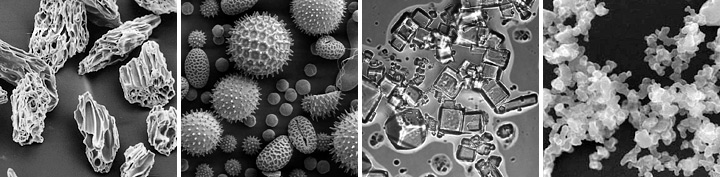
\includegraphics[width=1.0\textwidth]{aerosol_micrographs.jpg}
    \caption{Image au microscope électronique à balayage, à des échelles différentes,
        illustrant la diversité de forme des aérosols.
        De gauche à droite : cendre volcanic, pollen, sel de mer et suie. Micrographies de
        l'USGS, UMBC (Chere Petty) et de l'Arizona State University (Peter Buseck). 
        Crédit : NASA earthobservatory \url{https://earthobservatory.nasa.gov/Features/Aerosols/}.
    }
    \label{fig:micrography}
\end{figure}

\subsection{Composition chimique}%
\label{ssub:composition_chimique}

En terme d'élements constitutifs de ces PM, il est d'usage de regrouper les espèces en
différentes classes représentant les espèces majeurs de la masse des PM. La
Figure~\ref{fig:chapter01/composition_chimique} présentes les gammes de concentrations
observée à travers le monde pour différentes typologies de site de prélèvement.
On y trouve différents ions issus de la condensation de la phase gaseuse (nitrate \NOt, formé à
partir des \ce{NO_x} et l'ammonium \ce{NH_4^+}, formé à partir de \ce{NH3}) et du sulfate
\SOq, formé par condensation du \ce{SO2} mais également émis par les volcans et les
activités anthropiques).
Une part également importante de la masse provient de la matière carbonnée, notée ici
carbone organic (ou \textit{organic carbon} OC). Ce terme regroupe un nombre extrèmement
important d'espèce chimique comportant une chaine carbonnée, de l'oxygène et
de l'azote. On y retrouve par exemple la cellulose ou autres sucres issues de sa
dégradation par combustion (lévoglucosan, mannosan, galactosan), des "polyols" (arabitol,
mannitol, etc) émis par les bactéries ou champignons~\autocite{samakePolyols2019}, ou encore
d'autres famille de molécule comme les alcanes, hopanes, composé aromatique polycyclique
ou même pesticide. Cette matière carbonnée est souvent exprimée en terme de matière
organique (MO, ou \textit{organic matter} OM) prennant en compte la masse du carbone mais
également des autres atomes (oxygène, azote…) via un facteur correctif variant entre 1.2
et 2.3 suivant les lieux de prélèvement.
Mais le carbone est également présent sous forme plus "pure" (i.e. sans oxygène ni azote).
On parle alors de carbon élementaire (\textit{elementary carbon} EC) lorsqu'il est mesuré
par méthode thermique, et de carbone noir (\textit{black carbon} BC) lorsqu'il est mesuré
par methode optique. Cette distinction EC ou BC provient du fait qu'il existe un continuum
entre le carbone organique et le carbone élémentaire, et que chacune des méthodes
d'observation implique une seuil de différentiation entre les deux catégories.
Finallement, d'autres ions sont également présents, comme le sodium \ce{Na^+}, le chlore
\ce{Cl-}, le magnésium \ce{Mg^2+}, etc. mais également de nombreux éléments métaliques
comme le cuivre \ce{Cu}, l'aluminium \ce{Al}, le titan \ce{Ti}, le calcium \ce{Ca}, le fer
\ce{Fe}, etc.

La composition chimique d'un aérosols dépend de ses sources d'émissions (voir
également~\ref{sec:signature_chimique_des_sources_demissions} mais également des
différents processus bio-physico-chimiques présents dans l'atmosphère. En effet, sous
l'effet des radiations solaires, de la capacité oxydante de l'atmosphère ou des
micro-organismes vivant dans l'air, la composition chimique des aérosols évolue au court
de sa vie. On parle d'\textit{aérosol primaire} lorsque le chimie reflète celle des
sources d'émission, et d'\textit{aérosol secondaire} lorsque les composés chimiques
proviennent de réactions ayant eu lieu dans l'air.

Cette sensibilié aux sources d'émissions explique en partie la variabilité observée sur
la composition chimique et sa sensibilité à la typologie du site de d'étude. Les sites
marins présentant d'avantage de sels marins, les sites proches des déserts de sable
d'avantage de poussière minérale, les sites urbains d'avantage de marqueur de combustion
(EC), etc.

\begin{figure}[htpb]
    \centering
    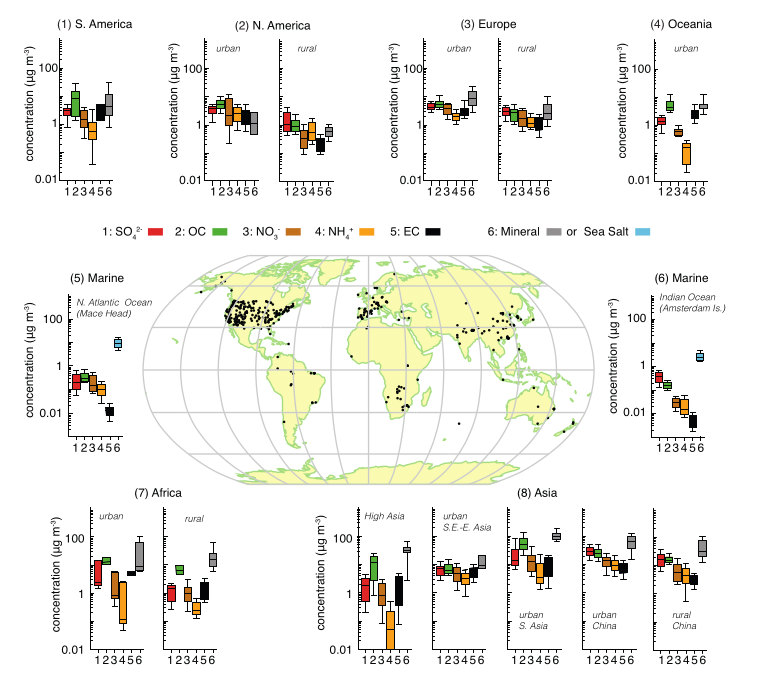
\includegraphics[width=1.0\linewidth]{chapter01/composition_chimique.png}
    \caption{Composition chimique majeurs de la masse des \PMdix{} pour différentes
        typologies de sites de prélèvement. Crédit: \cite[figure 7.13]{boucherClouds2013},
        aggrégeant 113 études sur au moins une année de prélèvement, entre 1993 et 2012.}%
    \label{fig:chapter01/composition_chimique}
\end{figure}

\subsection{Impacts climatiques des aérosols}%
\label{sub:impacts_climatiques_des_aerosols}

Les aérosols sont un éléments essentiels de la machine climatique terrestre de part leur
interraction avec le rayonnement solaire et donc leur impact sur le bilan radiatif de la
Terre, mais également par leur interraction très forte avec la dynamique des nuages, au
point que les rapports du GIEC traitent dans le même chapitre les nuages et les aérosols.

\paragraph{Impact radiatif}%
\label{par:impact_radiatif}

De part leur faible taille, les aérosols diffusent le rayonnement incidant et agisent donc
comme "bouclier thermique", ré-émettant une partie du flux solaire entrant dans l'espace,
conduissant ainsi à un refroidissement de l'atmosphère.
Cependant, les aérosols absorbent aussi une partie du rayonnement incidant, augmentant
l'agitation thermique et donc conduissant à un réchauffement du climat.
Ces deux effets agissent de concert, à différentes altitudes de l'atmosphère, et selon la
composition chimique des aérosols.
Enfin, la déposition des aérosols, et notamment du black carbone, sur la neige ou les
glaces des banquises induit un effet bien connu de rétroaction possitive : le carbone
absorbant le rayonnement normalement réémis par les surfaces blanches diminue l'albédo de
la surface, augmente localement la température, fait fondre la glace, découvrant des
surfaces plus sombre (roche ou océan), absorbant d'avantage de rayonnement, conduisant à
un réchauffement accrue, etc.

\paragraph{Noyaux de condensation des nuages}%
\label{par:noyaux_de_condensation_des_nuages}

Mais les aérosols, grâce à leur taille et leur ions, permettent également de baisser
l'énergie d'activation nécessaire à l'aggregation de la vapeur d'eau sous forme liquide en
goutelettes, puis goutte, facilitant l'apparition des nuages. Ainsi, les aérosols agissent
comme noyaux de condensation des nuages (CCN pour \textit{cloud condensation nuclei}). Or
les nuages empèches certes les infrarouges terrestres de repartir vers l'espace, mais
présentent également un albédo élevé, renvoyant une grande partie du rayonnement à courte
longueur d'onde du soleil vers l'espace. L'effet observé est donc un refroidissement du
climat.
Aussi, pour une même quantité d'eau, le nombre de CCN disponible conditionne la taille des
goutellettes des nuages, et donc leur taille, durée de vie et probabilité de se
transformer en nuage précipitant.

\paragraph{Impacts sur le déréglement climatique en cours}%
\label{par:impacts_sur_le_dereglement_climatique_en_cours}

Pour ces différents aspects, très brievement exprimé ici, l'impact total des aérosols sur
le climat est connu avec une incertitude élevée. 

Notamment, leur contribution à la différence du forcage radiatif entre 1750 et 2011 --qui
est de \SI{2.29}{\W\m\squared}-- s'estime entre
\SIrange[range-phrase=~et~]{-0.77}{0.23}{\W\per\m\squared}, avec un forçage négatif pour
les poussières minérale, le sulfate, nitrate et carbonne organique, mais positif pour le
carbonne noir.  Quant à leur rôle sur la dynamique des nuages, il s'estime entre
\SIrange[range-phrase=~et~]{-1.33}{-0.06}{\W\per\m\squared}, mais présente des
incertitudes plus élevés dû fait de la complexité à prendre en compte ces phénomènes dans
les modèles de climat. C'est actuellement le forcage radiatif le moins bien connu de la
machine climatique Terrestre.

\subsection{Impacts environnementaux}%
\label{sub:impacts_environnementaux}

La durée de vie des aérosols dans l'atmophère entre leur émission et leur déposition est
de plusieurs jours. Dans ce délai, la circulation atmosphérique les déplacent sur des
distance pouvant être de plusieurs milier de kilomètre. Il n'est pas rare par exemple en
Europe d'avoir des épisodes de dépositions de sable provenant du désert saharien. Ce
déplacement longue distance d'aérosols est même un des mécanismes clef de certains "bloom"
de phytoplancton, apportant d'importante quantité de nutriment à la surface de l'océan (en
métaux et phosphate notamment).
Plus spectaculaire, les cendres volcaniques relarguées dans l'atmosphère suite à de
violentes éruptions, en plus de leur impact climatique potentiel, peuvent occasioner des
pluies acides du fait de la présence en quantité de sulfate dans ces cendres.
Autre exemple marquant, le nitrate est l'un des éléments limitant de la croissance des
plante en prairie d'altitude. Or une partie importante de ce nitrate est apporté par
déposition de nitrate d'amonium particulaire provenant du transport longue distance.

Cette liste n'a pas pour but d'être exhaustif mais uniquement de présenter à quel point
les aérosols et leur composition chimique variée impacte directement de nombreux
écosystèmes terrestres, qu'ils proviennent de source anthropiques comme c'est le cas pour le
nitrate, ou de sources naturelles.

\subsection{Impacts sanitaires}%
\label{sub:impacts_sanitaires}

Finallement, l'impact sanitaire des aérosols sur la population humaine a commencé à être
un sujet de recherche suite à l'industrialisation et aux épisodes de "smog" causant la
mort de plusieurs personnes à Engis (Meuse, Belgique) en 1930, Donora (Pennsilvanie, USA)
en 1948 ou encore le plus connu "Great smog of London", en 1952. Durant ces épisodes de
polutions, il est important de noter que la sur-mortalité due à l'exposition aigue durant
l'épisode de pollution est très importante (jusqu'à 3 fois supérieure à la normale pour le
smog de Londre), mais que la surmortalité persiste dans les mois qui suivent --pendant
près d'un an pour le smog de Londre, alors même que les niveaux de pollutions étaient
revenus à leurs états pré-décembre 1952 \autocite{bellReassessment2001}.
Ces épisodes de pollutions intenses marquent le début de la prise de conscience de la
population de la problématique de la pollution de l'air et on conduit à la première
legislation anglaise en matière de qualité de l'air en 1956 avec le \textit{Clean Air
Act}. Aussi, des programmes de mesures de la qualité de l'air pour différents polluants
ont émergés et les actions misent en œuvre au niveau national et international ont permis
en Europe une amélioration très sensible de la qualité de l'air (Figure~\ref{fig:chapter01/tendance_polluants}).

\begin{figure}[ht]
    \centering
    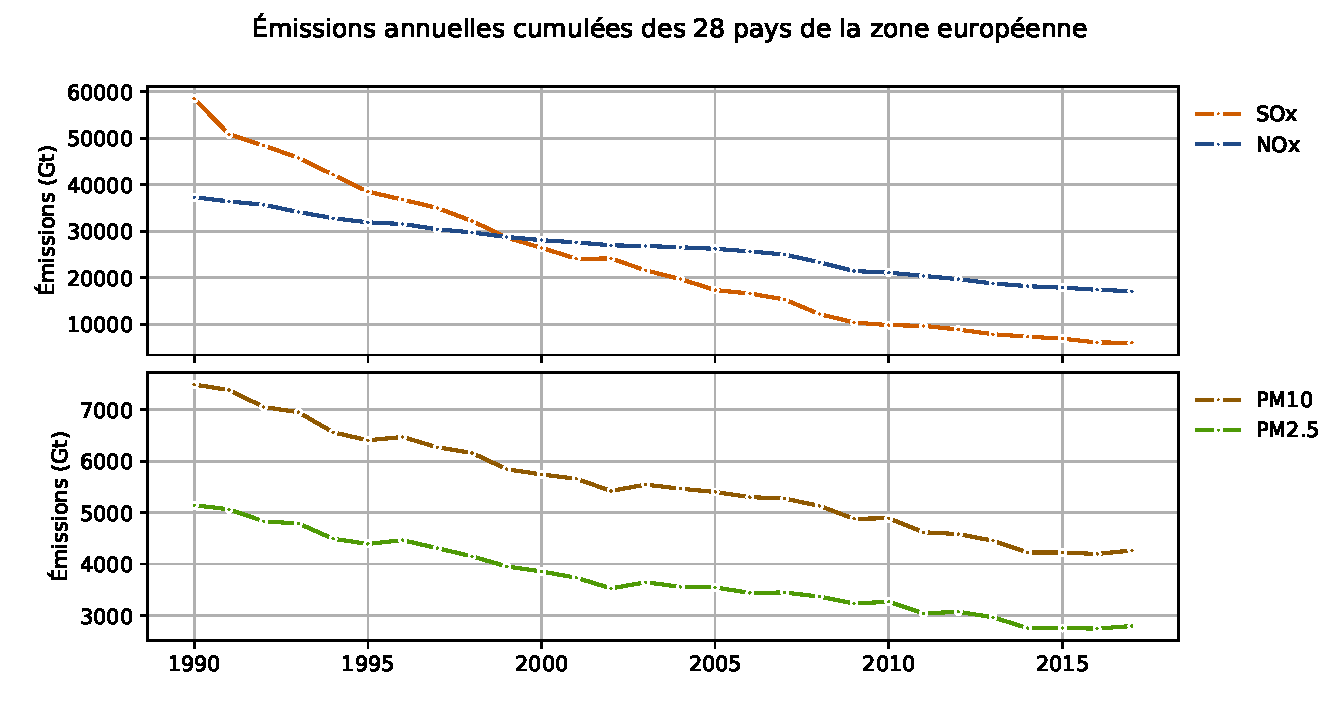
\includegraphics[width=0.9\linewidth]{chapter01/tendance_polluants.pdf}
    \caption{Évolution temporelle des émissions cumulés des 28 pays de la zone européenne
    depuis 1990, indiquant une prise de conscience et une diminution des émissions de
différents polluants gaseaux (SOx et NOx) et particulaire (\PMdix{} et \PMdc). Données
issues de \textit{National emissions reported to the Convention on Long-range
Transboundary Air Pollution (LRTAP Convention)}, ©European Environment Agency (EEA).}%
\label{fig:chapter01/tendance_polluants}
\end{figure}


Cependant, la qualité de l'air (incluant les aérosols, mais également les
composés gaseux comme les \ce{NO_x} ou l'ozone) demeure actuellement la 5\ieme{} cause de
mortalité dans le monde, représente un décés sur dix et est catégorisé "cancérogène
certain" par le CIRC depuis 2013. En Europe, pour l'année 2013, c'est
ainsi \num{800000} personnes qui sont décédés des suites de maladies cardiovasculaires,
cancer, pneumonie… directement imputable à la qualité de l'air
\autocite{worldhealthorganizationAmbient2016}.
En terme de bilan financier, la banque mondiale en collaboration avec l'Institute for
Health Metrics and Evaluation (IHME) de l'université de Washington estimait que le coût
associé aux décés prématurés de la seule année 2013 s'évaluait à plus de \$5.11 trillion
de dollar dans le monde~\autocite{worldbankCost2016}.

Afin de limiter cet impact sanitaire, de nombreux pays ont définis des seuils de
concentrations de différents composés. Seulement ces seuils sont différents d'une
institution à une autre. Par exemple, entre 2015 et 2017, le seuil de concentration
journalière recommandé pour les \PMdix{} par l'union européenne (\SI{50}{\ugm} en moyenne
journalière) était dépassé pour entre 13 et 19~\% de la population européenne, mais cette
proportion augmente à entre 42 et 62~\% si l'on prend en compte le seuil recommandé de
l'OMS de \SI{20}{\ugm} en moyenne annuelle~\autocite{europeanenvironmentagencyAir2019}.
De plus, il est à noter qu'il n'existe pas de seuil à partir duquel l'exposition aux PM
est inofensif.

\section{Détermination des sources d'émission des PM}%
\label{sec:source_apportionment_of_pm}

Comme nous l'avons vu, les sources d'aérosols sont très diverses.
Afin de pouvoir avoir un impact sur les concentrations de polluants, il est primordial de
retracer leur provenance. Plusieurs techniques d'analyses existe, qu'elles soient purement
physique ou géochimique.

\subsection{Signature chimique des sources d'émissions}%
\label{sec:signature_chimique_des_sources_demissions}

Chaque source d'émission n'émettant pas les mêmes composés, une analyses chimiques
des PM permet l'estimation des contributions des différentes sources aux PM observées.
Seulement, il n'est pas possible de mesurer l'entièreté des plus de 1000 espèces chimiques présentes
dans les aérosols.
Il convient donc de connaître au mieux la signature chimique des différentes sources
d'émissions, notamment via des prélèvements à l'émission en condition
réelle ou en chambre d'étude. La connaissance des espèces spécifiquement émises ou des
ratio d'émissions entre différentes espèces des différentes sources permetront par la
suite l'attribution de la contribution de ces sources aux PM observés.

\subsubsection{Analyse chimique des particules fines}%
\label{ssub:analyse_chimique_des_particules_fines}

Les données utilisées pour cette thèse proviennent d'analyse faite en laboratoire à
partir de prélèvement de terrain (mesure \textit{off-line}) via des préleveurs
automatiques haut-volume, selon les recommandations de
l'EN~16450:2017~\autocite{cenAmbient2017a}, chaque prélèvement correspondant à une
journée d'échantillage. Les prélèvements étant réalisé sur des filtres en fibre de quartz
pré-chauffée, grâce à un préleveur haut-débit (\SI{30}{\cubic\m\per\hour}) DA80 digitel.
La fraction prélevée correspond toujours aux \PMdix{}.

Dans les espèces courrament analysés et utilisés durant cette thèse, on retrouve :

\begin{description}
    \item[OC et EC] le carbone organique et élémentaire, mesuré par méthode
        thermo-optique~\autocite[Sunset Lab. Analyser]{birchElemental1996}, par le
        protocole EUSAAR-2~\autocite{cavalliStandardised2010,cenAmbient2017a};

    \item[Ions] \ce{Cl-}, \ce{NO3^-}, \ce{SO4^2-}, \ce{NH4+}, \ce{Na+}, \ce{K+},
        \ce{Mg^2+}, \ce{Ca^2+} et acide methane suflonique (MSA), déterminés par
        chromatographie ionique~\autocite{jaffrezoSeasonal2005,cenAmbient2017b};

    \item[Métaux et éléments traces] Al, Ag, As, Ba, Be, Br, Bi, Ca, Cd, Ce, Co, Cr, Cs,
        Cu, Fe, K, La, Li, Mg, Mn, Mo, Na, Ni, Pb, Pd, Pt, Rb, Sb, Sc, Se, Sn, Sr, Ti, V,
        Zn et Zr, mesurés par ICP-AES ou
        ICP-MS~\autocite{allemanPM102010,mbengueSizedistributed2014,cenAmbient2005}

    \item[Monosacharides] Levoglucosan, mannosan, galactosan, arabitol, manitol, sorbitol
        et glucose, analysés par
        HPLC-PAD~\autocite{piotQuantification2012,wakedSource2014}.

\end{description}

\subsubsection{Profile chimique des sources d'émissions courrante}%
\label{ssub:profile_chimique_des_sources_d_émissions_courrante}

\begin{description}
    \item[Combustion de biomasse] provenant en Europe majoritairement du chauffage
        domestique. Le type de combustible et les conditions de combustion influence
        grandement sur les espèces chimiques émises. On retrouve cependant toujours de
        l'OC en grande quantité, ainsi que de l'EC. Aussi, si le BC est mesuré, il est
        possible d'estimer la part du BC provenant de cette source de combustion \BCwb{}
        (\textit{BC wood burning}).
        Provennant de la pyrolyse de la cellulose, le lévoglucosan, mannosan et
        galactosan forment 3 proxy spécifique de cette source car il n'existe pas d'autre
        procédé connu conduisant à leur présence dans l'atmosphère que la combustion de
        bois~\autocite{jordanLevoglucosan2006,puxbaumLevoglucosan2007}.
        Enfin, du potassium \ce{K+} et du rubidium Rb sont également associés à cette
        source~\autocite{navaBiomass2015,gollyEtude2014,chevrierChauffage2016}.

    \item[Traffic routier] émettant différents métaux (Ca, Cu, Mo, Pb, Sb, Sn, Fe, Zr,
        Ti) et de la matière carbonnée --notamment de l'EC-- et des composés organiques
        (hopanes, alcanes)~\autocite{schauerCharacterization2006,charronIdentification2019}. Les émissions
        véhiculaires sont parfois séparées en 2 sous-types : émissions à l'échappement
        provenant de la combustion~\autocite{allenSize2001,huMetals2009,vianaSource2008},
        et émissions hors-échappement (abrasion de la route, usure des freins et pneus,
        etc.)~\autocite{grigoratosBrake2015,sandersAirborne2003,sternbeckMetal2002}.

    \item[Émission primaire biogenique] directement émise par les micro-organismes du sol
        et des plantes, qui, de par leur activité biologique, émettent notamment
        différents polyols : arabitol, mannitol,
        sorbitol~\autocite{bauerSignificant2008,yttriAmbient2007,samakePolyols2019}.

    \item[Poussière crustale] remise en suspension par le vent ou les activités humaines
        (mine, carrière, etc). Ce profile chimique reflète celui de la croute continental
        et présente donc du \ce{Mg^2+}, \ce{Ca^2+}, Ti, Mn et Fe, mais très peu de composés
        organiques~\autocite{almeidaSource2005,dallostoHourly2013,morenoVariations2011,putaudSizesegregated2004}.

    \item[Sel de mer] issue des embruns marins, présentant donc une grande proportion de
        \ce{Na+} et \ce{Cl-}, mais également de
        \ce{Mg^2+}~\autocite{belisCritical2013,odowdMarine1997,pioClimatology2007}. Il
        est à noter que le sel de route, notamment en vallée alpines, présente la même
        composition chimique~\autocite{airrhone-alpesInfluence2012}.

    \item[Industrie] Les profiles chimiques des sources industrielles sont très variables
        car dépendent directement du type d'industrie. Cependant, il est courrant d'y
        retrouver des métaux, du \SOq et certains composés organiques spécifique (HAP et
        HAPs, hopanes...) selon les procédés
        industriels~\autocite{sylvestreComprehensive2017}.

    \item[Port et bateau] proche des côtes notamment. Marqué par la présence de V et Ni,
        provenant de la combustion de fuel lourd, mais également de composés organiques
        comme les hopanes.

    \item[Agriculture] émettant notamment du nitrate et de l'ammoniac à travers les
        fertilisant de synthèse ou de fumier. Cette source d'émission est notamment
        responsable des pics de pollution printanier, lors des épendages agricole à cette
        période.

    \item[Volcan] beaucoup plus ponctuel --surtout en Europe-- mais néanmoins possible
        (par exemple l'Eyjafjöll en 2010), les volcans émettent de grand quantité de
        poussère minérale et d'éléments traces, mais également de soufre et donc de \SOq.

\end{description}

\subsubsection{"Sources" secondaires}%
\label{ssub:_sources_secondaires}

Aux sources primaires précédemment listées, il faut ajouter les processus secondaires lié
à la photochimie ou au vieillissement des aérosols, qui conduisent à la formation de
nouvelles espèces chimiques.

\paragraph{Aérosol organique secondaire}%
\label{par:aérosol_organique_secondaire}

Notamment, la biologie est connue pour émettre du dimethyl sulfate (DMS), s'oxydant en
MSA dans l'atmosphère. Sa présence dans les PM trace donc le viellissement d'un aérosol
d'origine organique.  L'oxalate est également un composé issue de réaction photochimique,
mais la diversité des composés primaires et voie de réaction rend extrêmement difficile
l'identification de la source originelle.
On nomme alors ces aérosols \textit{secondary organic aerosol} (SOA), dont le
dénominateur commun est de présenter une fraction importante de matière organique
oxygéné. Il est compliqué avec des analyses moléculaire d'en déterminer l'origine et des
travaux sont en cours en ce sens et présenté dans le chapitre~\ref{chap:todo}.

Il faut noter que d'autres techniques d'analyses, notamment l'ACSM, permettent une
analyse plus avancée de cette fraction organique de l'aérosols, sans pour autant pouvoir
caractériser moléculairement les éléments retrouvés.

\paragraph{Aérosols inorganique secondaire}%
\label{par:aérosols_inorganique_secondaire}

Mais la partie organique n'est pas la seul à réagire dans l'atmopshère. Ainsi, les NOx,
gaseux, émis notamment par le transport routier, peuvent condensé en phase particulaire
lorsqu'ils s'associent à l'ammoniac, provenant du secteur agricole, pour former du
nitrate d'ammonium \ce{NO3NH4}. Il en est de même pour le \ce{SO2} émis par différentes
sources ou des fonctions sulfatés de la matière organique, et l'ammoniac, condensant en
sulfate d'ammonium \ce{SO4(NH4)2}.

\paragraph{Vieillissement et volatilité}%
\label{par:vieillissement_et_volatilité}

Aussi, la partie la plus volatile de la phase particulaire tend à s'évaporer et rejoindre
la phase gaseuse au cours du temps. C'est ainsi qu'après plusieurs jours de transport
dans l'atmopshère, le sel de mer peut avoir ''dégasé'' le chlore présent dans son réseau
cristallin, et présenté des substitution avec du sulfate ou du nitrate. De même que la
sodium peut avoir été remplacé par d'autre cations comme le potassium ou le magnésium.
Souvent, ce procédé est associé a une augmentation de la matière organique liée à cet
aérosol.

\subsection{Modèle d'attribution des sources}%
\label{sec:source_apportionment_model}

Afin d'estimer la contribution de chaques sources de PM à un point donnée, il est possible
d'utiliser 2 grandes familles de modèles d'attribution des sources (\textit{source
apportionment} (SA)). La première est fondée sur notre connaissance des
émissions et de la météorologie et calcul les réactions physico chimique depuis les
sources jusqu'au lieu d'étude (modèle dit de chimie-transport (\textit{chemical transport
model} (CTM)) alors que la deuxième s'evertue à mesurer en un point donné
la chimie des PM et par traitement statistique, attribue a différente source ou
''facteur'' leur contribution aux concentrations observées (modèle dit récepteur
(\textit{receptor model} RM)).

\subsubsection{Modèle déterministe de chimie-transport}%
\label{ssub:modele_deterministe_de_chimietransport}

\paragraph{Présentation}%
\label{par:presentation}

Les modèles déterministes s'appuient sur l'inventaire des sources d'émissions sur la
région étudiée. Ces cadastres d'émissions sont regroupés en catégorie \textit{Selected
Nomenclature for reporting of Air Pollutants} (SNAP) représentant chacune un secteur
d'activité : Énergie, Procédés industriel, Agriculture, Déchets, Autres et enfin
Naturelle.
Chacune de ces catégories possèdent évidemment des sous-catégories raffinant la
classification (par exemple, les émissions de l'aviation civile de plus de \SI{100}{m} de
long se retrouvent dans le SNAP 080503 (ou \textit{Nomenclature For Reporting} (NFR)
1.3.A.c) autrement dit Énergie - Combustion - Aviation - Aviation civile de plus de
\SI{100}{m})~\autocite{europeanenvironmentagencyEMEP2019}.
À chacun de ces SNAP est associé un profile d'émission (\ce{O3}, \ce{SO2}, NOx, \ce{NH3}, \PMdix, \PMdc,
VOC principallement).

Vient ensuite un inventaire de ces sources d'émissions sous forme de cadastre géographique
et temporelle. Notamment la \textit{Convention on Long-Range Transboundary Air
Pollution} (LRTAP) implémenté par l'\textit{European Monitoring and Evaluation Program}
(EMEP) sous l'égide de \textit{United Nations Economic Commission for Europe} (UNECE),
prévoit que les différentes parties prennante à cette convention présentent un rapport de
leurs émissions régulièrement à l'EMEP.

Ainsi, il est alors possible de construire des modèles déterministes de dispersion et de
réaction des polluants, en couplant un modèle de diffusion résolvant les équations de la
physique de l'atmosphère avec un modèle physico-chimique faisant évoluer les composés
gaseux et particulaires, incluant leurs émissions, dépots, interraction physico-chimique,
etc. Pour n'en citer que quelqu'uns : 
Community Multi-scale Air Quality (CMAQ)\footnote{\url{https://www.epa.gov/cmaq}},
Comprehensive Air Quality Model with Extensions (CAMx)\footnote{\url{http://www.camx.com/}},
WRF-Chem\footnote{\url{https://www2.acom.ucar.edu/wrf-chem}},
Chimère,
LOTOS-EUROS...

La raison de la pluralité de ces modèles provient des différentes paramètrisations
possibles des équations physiques, mais également des choix conceptuels de recherche.

\paragraph{Source apportionment}%
\label{par:source_apportionment}

Concernant l'attribution des sources, il est possible d'utiliser deux techniques au sein
des CTM:

\begin{enumerate}
    \item Faire une première simulation incluant toutes les sources d'émissions, puis une
        deuxième avec une source en moins. La différence reflettant l'impacte de la source
        supprimée sur les concentrations ambiantes ;
    \item Tracer la provenance de chacunes espèces chimiques lors des schéma réactionnels
        (\textit{source labelling} ou \textit{tagged species}).
\end{enumerate}

Seulement, du fait des nombreux processus non linéaire, la suppression d'une source
d'émission aura des répercussions beaucoup plus complexe que la simple diminution des
concentrations propre à cette source (par exemple, des NOx pouraient ne pas passer en
phase particulaire du fait d'un manque d'ammoniac). La première solution correspond donc à
se demander 
\begin{quote}
    Si je diminue ou supprime les émissions de cette source, quels impacts cela va-t-il
    avoir sur les concentrations ?
\end{quote}
alors que la deuxième répond à
\begin{quote}
    Dans la concentration ambiante, à combien s'estime la contribution de telle source
    d'émission ?
\end{quote}
Cette dernière technique a commencé été implémenté plus récemment dans certains
CTM~\autocite{wangDevelopment2009,wagstromDevelopment2008,kranenburgSource2013,brandtContribution2013}
et détaillé dans le rapport de~\textcite{mirceaEuropean2020}.

Cependant l'utilisation des CTM présente certaines limites du fait de leur complexité.
Notament, il semble illusoire de pouvoir un jour inclure toutes les réactions chimiques
possibles dans les modèles déterministe, et quand bien même ce serait le cas --car les
modèles réactionnels sont de plus en plus poussé--, il faudrait alors avoir des
inventaires d'émissions beaucoup plus complet et précis temporellement, avec aucune
certitude d'un oublie potentiel d'une source non prise en compte.  Aussi, la limitation
physique des modèles météorologiques se retrouvent dans les CTM. Il est donc compliqué
d'envisager, du fait du coût de calcul et de stockage, une simulation à \SI{10}{m} de
résolution spatiale (ou moins), ce qui serait cependant nécessaire pour apréhender
correctement des phénomènes précis, comme les inversions thermiques des vallées alpines.

\subsubsection{Modèle récepteur}%
\label{ssub:model_recepteur}

À l'inverse, il est possible d'estimer les sources contribuant aux concentrations
ambiantes en un lieu donné sans la moindre information météorologique ou simulation
déterministe. Pour cela, il convient de faire des prélèvements sur le lieu d'étude,
d'analyser la chimie que l'on y trouve, et à l'aide de modèle statistique, de retrouver
les différents profiles de source et leur contribution, traduisible pas l'équation
d'équilibre des masses
\begin{align}
    \label{eq:mass_balance}
    X &= G \cdot F
\end{align}
où $X$ est la matrice de dimension $n\times m$ des observations, $G$ est la matrice des
contribution de taille $n\times p$ et $F$ la matrice des profiles de taille $p \times n$,
avec $n$ le nombre d'échantillon, $m$ le nombre de variables chimiques mesurées et $p$ le
nombre de facteur. Un facteur peut être une source d'émission (combustion de biomasse par
exemple), mais également regrouper des espèces chimiques provenant d'un même processus
secondaire (nitrate d'ammonium par exemple).
Il est courrant d'exprimer $X$ en \si{\ugm}, $G$ en \si{\ugm} ou concentration
normalisée~\si{[-]} et $F$ en \si{\micro\g\per\micro\g} ou \si{\ugm}.

Si l'on mesure $X$, ce qui nous intéresse ici est de connaître $G$ et/ou $F$. Si l'on
admet que l'on connait a priori les profiles d'émission possibles, alors $F$ est connu, et
l'on cherche à estimer $G$. Le modèle de déconvolution adapté est alors le
\textit{Chemical Mass Balance} (CMB). À l'opposé, on peut n'avoir aucune information a
priori à la fois sur les contributions et les profiles d'émissions. On utilisera alors le
modèle de déconvolution \textit{Positive Matrix Factorization} (PMF).  Ces 2 types de
modèles statistiques sont aux deux extrèmes d'un spectre de modèle statistique depuis une
information ''absolue'' des profiles de sources à une absence totale d'information de ces
mêmes profiles.  Il existe cependant un continuum entre ces deux pôles (voir
Figure~\ref{fig:chapter01/source_apportionment_methods}, et de nombreux modèles ont été
développé et amélioré depuis la première étude de SA de \textcite{colucciAutomotive1965}
utilisant la ''simple'' corrélation entre le \ce{CO} et le plomb et benzo(a)pyrène.  Une
revue détaillée et historique du fonctionnement de ces différents modèles peut-être
retrouvé sur les articles de
\textcite{henryHistory1997,vianaSource2008,belisCritical2013,hopkeReview2016}.

\begin{figure}[ht]
    \centering
    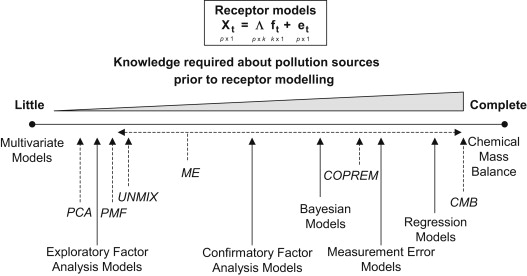
\includegraphics[width=0.6\linewidth]{chapter01/source_apportionment_methods.png}
    \caption{
        Connaissance a priori nécessaire pour les différents modèles de SA existant,
        depuis la simple analyse de facteur par ACP au modèle CMB. Crédit :
        \textcite{vianaSource2008} adaptée de \textcite{schauerCharacterization2006}
    }%
    \label{fig:chapter01/source_apportionment_methods}
\end{figure}

Dans cette thèse, seul le modèle PMF résolue grâce au solver ME-2 développé par
\textcite{paateroMultilinear1999} a été utilisé, et va maintenant être décrit en détail.

\subsubsection{Modèle source récepteur PMF}%
\label{ssub:pmf}


\section{Vers une mesure unifiée: le potentiel oxydant}%
\label{sec:le_potentiel_oxydant_des_aerosols}

Devant la grande variété de chimie, forme, taille, etc. des aérosols, il apparaît
compliqué de résumer la toxicité de l'air que l'on respire à sa simple concentration
massique en aérosols. En effet, il est évident que respirer un~\si{\ugm} de sable n'aura
pas le même impact sur notre santé qu'un~\si{\ugm} de mercure ou de plomb.  Seulement, la
mesure massique est l'une des plus simples a implémenter en routine et est également
facilement automatisable, permettant ainsi un premier ordre de grandeur de l'exposition
des populations. Aussi, il est important de rappeler que les aérosols n'ont pas qu'un
impacte sanitaire, mais également climatique (voir
section~\ref{sub:impacts_climatiques_des_aerosols}), pour lequel la messure de la
concentration est tout a fait adaptée.

Afin de répondre à ce problème, il a été proposé dans les années 2010 une nouvelle mesure,
intégratrice des propriétés physico-chimique des aérosols, sensé être plus proche des
impacte sanitaire occasioné par les PM. En effet, un des mécanismes suspecté d'être à
l'origine des troubles sanitaires engendrés par les aérosols est le stresse oxydatif
induit lors de l'inhalation des particules, entrainant une cascade de réaction au sain de
notre organisme.
Cette nouvelle mesure tente de quantifier les espèces réactive de l'oxygène (ROS) présente
ou induite par les aérosols en mettant en contact les aérosols et un antioxydant.
Le suivit de la cinétique de la réaction permet ainsi d'estimer la réactivité de la
particule, prenant en compte non seulement sa chimie, mais aussi la taille et forme des
particules à travers leurs surface de réaction et également les potentiels "effet
cocktail" lors de la combinaison de différentes espèces chimiques.

\subsection{Methodologie de mesure}%
\label{sub:methodologie_de_mesure}

\subsubsection{Prendre en compte la bioaccessibilité: SLF}%
\label{sub:prendre_en_compte_la_bioaccessibilite_slf}

\subsubsection{Differents agent réactant}%
\label{ssub:differents_agent_reactant}

\paragraph{Mesure par Ditiothreitol}%
\label{ssub:mesure_par_ditiothreitol}

\autocite{choRedox2005}

But \autocite{beiReaction2014}

\paragraph{Mesure par Acide ascorbic}%
\label{ssub:mesure_par_acide_ascorbic}

\paragraph{Mesure par DCFH}%
\label{ssub:mesure_par_dcfh}

\paragraph{Autres methodes de mesure}%
\label{sub:autres_methodes_de_mesure}

\subsubsection{Unitées de mesures}%
\label{ssub:unitees_de_mesures}

La mesure du PO par DTT ou AA fournit une consomation de réactant en \si{\nano\mole\per\min}.
Cependant, cette mesure est nécessairement dépendante de la quantité de PM introduite dans
la réaction.
Il convient donc de normaliser cette consommation d'antioxydant par la masse des réactifs.
Seulement, cette mesure n'est pas fidèle à l'exposition des personnes car ne prend pas en
compte la concentration en particule. De ce fait, deux normalisations de la réactivité des
particules co-existent.

\paragraph{Normalisation par la masse}%
\label{par:normalisation_par_la_masse}
Pour exprimer la réactivité "intrinsèque" d'une particule, la cinétique de déplétion
d'antioxydant ($cAO$, en \si{\nmol\per\min}) est normalisée par la masse de réactif
introduit (en \si{\ug}). On obtient ainsi le PO par \si{\ug}, noté \OPm{} en
\si{\nmol\per\min\per\micro\g}:
\begin{align}
    \label{eq:opm}
    OP_m &= \frac{cAO - cAO_{blank}}{M}
\end{align}
où $cAO$ est la consommation d'antioxydant dans l'échantillon et $cAO_{blank}$
est la consommation d'antioxydant dans les blancs, tous deux en \si{\nmol\per\min}, et $M$
la masse de réactif introduit (PM ou élement chimique), en \si{\ug}.

\paragraph{Normalisation par le volume}%
\label{par:normalisation_par_le_volume}

Seulement, la réactivité intrinsèque n'est pas un indicateur propice à l'exposition. En
effet, il faut également tenir compte de la concentration ambiante des particules. Le PO
est donc aussi exprimé par unité de volume, notée \OPv{} en
\si{\nmol\per\min\per\cubic\meter} et parfois appelé PO "extrinsèque", calculé par:
\begin{align}
    \label{eq:opv}
    OP_v &= OP_m \times [\text{PM}]
\end{align}
où [PM] correspond à la concentration en particule en \si{\ugm}. Cette expression se
retrouve également écrite~\autocite{fangSemiautomated2015} sous la forme
\begin{align}
    \label{eq:opvalt}
    OP_v &= \frac{cAO - cAO_{blank}}{V}
\end{align}
où $V$ est le volume d'air analysé. Ces deux formes sont cependant équivalentes, car en
replacant $V = \frac{M}{[PM]}$ dans l'Eq.~\ref{eq:opvalt}, on retrouve bien
l'Eq.~\ref{eq:opv}:
\begin{align}
    \label{eq:opvopvalt}
    OP_v &= \frac{cAO -cAO_{blank}}{V} = \frac{cAO -cAO_{blank}}{M}\times [\text{PM}] = OP_m \times [\text{PM}].
\end{align}

\paragraph{Comparabilité des échantillons}%
\label{par:comparabilité_des_échantillons}

Le fait de se rammener à un microgramme de PM en divisant par la masse introduite fait
l'hypothèse d'une linéarité du PO en fonction de la masse. Hors, il a été montré par
\textcite{charrierDithiothreitol2012,charrierBias2016,calasComparison2018} que cette
hypothèse est fausse dans le test au DTT et qu'il présente en réalité une réponse
pseudo-logarithmique en fonction de la masse du réactif.

Ainsi, 2 analyses du même filtres ne présenteront pas la même valeur de \PODTTm{} si la
concentration en PM n'est pas identique, les analyses faites à ''fortes masses''
présenteront toujours un \PODTTm{} plus faible que celles à ''faibles masses''.
La comparabilité des échantillons n'est donc possible que si les annalyses sont faites à
masses constantes, ou artificiellement corrigées, soit par interpolation, soit par
estimation grâce à la concentration de Cu et Mg, comme le propose
\textcite{charrierBias2016}.

Il faut également noter que ce biai se propage au \PODTTv{} du fait de sa linéarité avec le
\PODTTm. Aussi, un deuxième biai apparaît ici. En effet, la non-linéarité du DTT fait
que la prolongation linéaire entre 1 microgramme et X microgrammes par mètre cube est
fausse. Le \PODTTv{} se comportant alors ''comme si'' les X microgrammes de PM de ce mètre
cube d'air se comportaient comme X fois 1/X 1 microgramme de PM, ce qui est faux de part
la non-linéarité du DTT.

Les analyses de \PODTT{} de cette thèse suivent donc le protocole défini lors de la thèse
de \textcite{calasPollution2017} : analyse à masse constante et faible de PM. Les
échantillons seront donc comparables entre eux. Le parti pris garder le biai
d'extrapolation de la ''faible masse'' à un volume d'air potentiellement charger en PM
pour le \PODTTv{} se justifie biologiquement par les faibles volume d'air présent dans les
poumons et donc la faible masse de PM en contacte avec les surfactants pulmonaires.

Une telles non-linéarité n'est pas observée pour les tests à l'acide ascorbique ou à la
DCFH.\todo{C'est vrai ca pour la DCFH ? On a checké ?}
Les résultats issus de ces tests sont donc à priori comparables entre les différentes
études.

\subsubsection{Conservation des échantillons et dérive temporelles}%
\label{ssub:conservation_des_échantillons_et_dérive_temporelles}

Les 

\subsection{État de la connaissance du PO}%
\label{sub:etat_de_la_connaissance_du_po}



\addcontentsline{toc}{section}{Bibliography}
\printbibliography[segment=2,heading=subbibliography]

\section{Positionnement de cette thèse}%
\label{sec:positionnement_de_cette_thèse}


